\documentclass[10pt]{article}
\usepackage[margin=.75in]{geometry} 
\usepackage{amsmath,amsthm,amssymb}
\usepackage{bm}
\usepackage{enumitem}
\usepackage{array}
\usepackage{lipsum}
\usepackage[]{units}
\usepackage{relsize}
\usepackage{tikz}
\usetikzlibrary{positioning}
\usepackage{graphicx}
\usepackage{xfrac}

\setenumerate{listparindent=\parindent}

\newcommand{\Q}{\mathbb{Q}}
\newcommand{\Z}{\mathbb{Z}}

\DeclareMathOperator*{\dom}{dom}
\DeclareMathOperator*{\Aut}{Aut}
\DeclareMathOperator*{\Gal}{Gal}

\def\slfrac#1#2{{\mathord{\mathchoice   % 
        {\kern.1em\raise.5ex\hbox{$\scriptstyle#1$}\kern-.1em
        /\kern-.15em\lower.25ex\hbox{$\scriptstyle#2$}}
        {\kern.1em\raise.5ex\hbox{$\scriptstyle#1$}\kern-.1em
        /\kern-.15em\lower.25ex\hbox{$\scriptstyle#2$}}
        {\kern.1em\raise.4ex\hbox{$\scriptscriptstyle#1$}\kern-.1em
        /\kern-.14em\lower.25ex\hbox{$\scriptscriptstyle#2$}}
        {\kern.1em\raise.2ex\hbox{$\scriptscriptstyle#1$}\kern-.1em
        /\kern-.1em\lower.25ex\hbox{$\scriptscriptstyle#2$}}}}}



\begin{document}

\begin{center}
\large Math 114 Homework 4

\normalsize Michael Knopf \\ February 26, 2014
\end{center}

Note: When an extension $K/F$ is Galois, its automorphism group $\Aut K/F$ is called the \emph{Galois group} of $K/F$ and is denoted $\Gal K/F$.  The \emph{Galois group} of a separable polynomial $p(X)$ over a field $F$ is defined to be the Galois group of any splitting field of $p(X)$ over $F$.  (See pp. 562-563 of DF.)

\begin{enumerate}

\item (Exercise 1 in DF \S 14.1.) Let $K/F$ be a finite extension.

(a) Show that if the field $K$ is generated over $F$ by the elements $\alpha_1,\ldots,\alpha_n \in K$, then an automorphism $\sigma$ of $K$ fixing $F$ is uniquely determined by $\sigma(\alpha_1),\ldots,\sigma(\alpha_n)$.  (That is, the values $\sigma(\alpha_1),\ldots,\sigma(\alpha_n)$ determine the value of $\sigma(\alpha)$ for every $\alpha \in K$.)

In particular, show that an automorphism of $K$ fixes $K$ if and only if it fixes a set of generators for $K$ over $F$.

\begin{proof}

Suppose $\sigma \in \Aut(K/F)$.  Since $K/F$ is a finite extension, it is algebraic.  Thus, for each $i$, $\alpha_i$ has some finite degree $k_i$, and a basis for $K$ over $F$ is $\{\alpha_1, \alpha_1^2, \dots, \alpha_1^{k_1}, \dots, \alpha_n, \alpha_n^2 \dots, \alpha_n^{k_n} \}$.

Let $\alpha \in K$.  Then there exist constants $a_{11}, a_{12}, \dots , a_{1k_1}, \dots , a_{n1}, a_{n2}, \dots , a_{n n_k}$ such that $\alpha = a_{11}\alpha_1 + a_{12}\alpha_1^2 + \cdots + a_{1k_1}\alpha_1^{k_1} + \cdots + a_{n1}\alpha_n + a_{n2}\alpha_n^2 + \cdots + a_{nk_n}\alpha^{k_n}$.  Therefore, since $\sigma$ is an automorphism fixing $K$, we must have
\begin{align*}
\sigma(\alpha) &= \sigma(a_{11}\alpha_1 + a_{12}\alpha_1^2 + \cdots + a_{1k_1}\alpha_1^{k_1} + \cdots + a_{n1}\alpha_n + a_{n2}\alpha_n^2 + \cdots + a_{nk_n}\alpha^{k_n})
\\
&= a_{11}\sigma(\alpha_1) + a_{12}\sigma(\alpha_1)^2 + \cdots + a_{1k_1}\sigma(\alpha_1)^{k_1} + \cdots + a_{n1}\sigma(\alpha_n) + a_{n2}\sigma(\alpha_n)^2 + \cdots + a_{nk_n}\sigma(\alpha)^{k_n}.
\end{align*}
So $\sigma$ is completely determined by its action on $\alpha_1, \dots , \alpha_n$.  If $\sigma$ fixes $\alpha_1, \dots , \alpha_n$, then $\sigma(\alpha) = \alpha$ for this arbitrary $\alpha$, thus $\sigma$ fixes $K$.  Clearly, if $\sigma$ does not fix some $\alpha_i$ then it does not fix $K$.

\end{proof}

(b) Let $G \leq \Gal(K/F)$ be a subgroup of the Galois group of the extension $K/F$ and suppose $\sigma_1,\ldots,\sigma_k$ are generators for $G$ (i.e., $G = \langle \sigma_1,\ldots,\sigma_k \rangle$).  Show that if $E$ is an intermediate subfield ($F \subset E \subset K$), then $E$ is fixed by $G$ if and only if it is fixed by the generators $\sigma_1,\ldots,\sigma_k$.

\begin{proof}

Clearly, if some $\sigma_i$ does not fix $E$ then $G$ does not fix $E$, since $\sigma_i \in G$.  Now, suppose $\sigma_i$ fixes $E$ for all $i$, and let $\sigma \in G$.  Then $\sigma = \sigma_1^{n_1} \circ \cdots \circ \sigma_k^{n_k}$ for some $n_1, \dots , n_k$.  Then for any $\alpha \in E$, we have
\begin{align*}
\sigma(\alpha) &= \sigma_1^{n_1} \circ \cdots \circ \sigma_k^{n_k}(\alpha) = \sigma_1^{n_1} \circ \cdots \circ \sigma_{k-1}^{n_{k-1}}(\sigma_n^{n_k}(\alpha))
\\
&= \sigma_1^{n_1} \circ \cdots \circ \sigma_{k-1}^{n_{k-1}}(\text{id}(\alpha)) = \sigma_1^{n_1} \circ \cdots \circ \sigma_{k-1}^{n_{k-1}}(\alpha)
\\
&= \cdots = \sigma_1^{n_1}(\alpha) = \alpha.
\end{align*}
So an arbitrary $\sigma \in G$ fixes an arbitrary $\alpha\in E$, thus $G$ fixes $E$.
\end{proof}

\item (Exercise 3 in DF \S 14.2.) Determine the Galois group of the polynomial $(X^2-2)(X^2-3)(X^2-5)$ over $\mathbf{Q}$.  Let $K$ be a splitting field for this polynomial over $\mathbf{Q}$; determine all the subfields of $K$.  (You may use the Galois correspondence, Theorem 14, although we haven't proved it in class yet.)

\begin{proof}

Let $p(x) = (x^2 - 2)(x^2 - 3)(x^2 - 5)$.  The splitting field $K$ for $p(x)$ over $\Q$ is $K = \Q(\sqrt{2}, \sqrt{3}, \sqrt{5})$.  A basis for $K$ as a vector space over $\Q$ is $\{1, \sqrt{2}, \sqrt{3}, \sqrt{5}, \sqrt{6}, \sqrt{10}, \sqrt{15}, \sqrt{30} \}$, therefore $[K:\Q] = 8 $.  Therefore, $\Gal(K/F) = \ <\sqrt{2} \mapsto -\sqrt{2}, \sqrt{3} \mapsto -\sqrt{3}, \sqrt{5} \mapsto -\sqrt{5}>$, because this group has order $8$ and we know that the maps generated by these are the only possible automorphisms of $K$ fixing $\Q$, since these are the only automorphisms that permute the roots of the irreducible polynomials $x^2 - 2$, $x^2 - 3$, and $x^2-5$.  The lattice of subfields of $K$ is drawn below.

\begin{figure}[h!]
\begin{center}
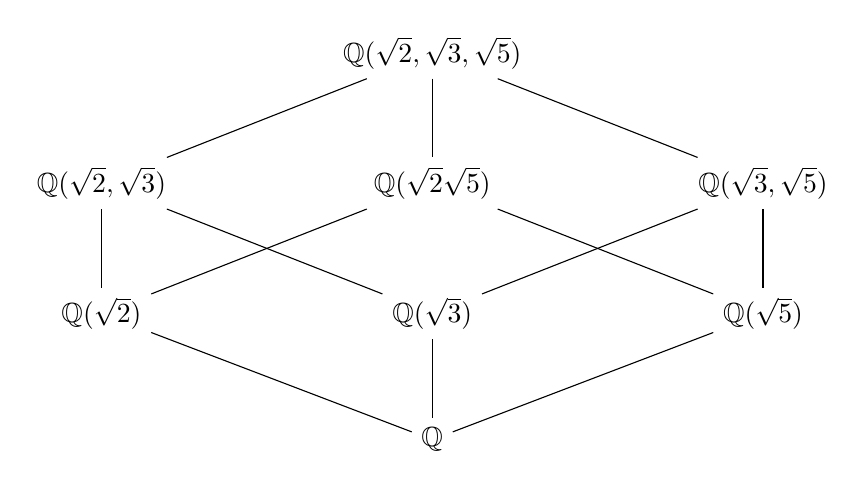
\begin{tikzpicture}[node distance=2cm]
\node(235) {$\Q(\sqrt{2},\sqrt{3},\sqrt{5})$};
\node(23)		[below left=1cm and 2cm of 235]
{$\Q(\sqrt{2},\sqrt{3})$};
\node(25)		[below =1cm of 235]
{$\Q(\sqrt{2}\sqrt{5})$};
\node(35)		[below right=1cm and 2cm of 235]
{$\Q(\sqrt{3},\sqrt{5})$};

\node(2)			[below =1cm of 23]
{$\Q(\sqrt{2})$};
\node(3)			[below =1cm of 25]
{$\Q(\sqrt{3})$};
\node(5)			[below =1cm of 35]
{$\Q(\sqrt{5})$};
\node(1)			[below =1cm of 3]
{$\Q$};

\draw(235) -- (23);
\draw(235) -- (25);
\draw(235) -- (35);
\draw(23)  -- (2);
\draw(23)  -- (3);
\draw(25)  -- (2);
\draw(25)  -- (5);
\draw(35)  -- (3);
\draw(35)  -- (5);
\draw(2)   -- (1);
\draw(3)   -- (1);
\draw(5)   -- (1);
\end{tikzpicture}
\end{center}
\end{figure}
\end{proof}

\pagebreak
\item (Exercise 4 in DF \S 14.2.) Let $p$ be a prime.  Determine the Galois group of $X^p-2$ over $\mathbf{Q}$.  (Hint: the example on p. 541 in \S 13.4 discusses the splitting field of this polynomial.  The example on pp. 577-579 in \S 14.2 may be useful as a model.)

\begin{proof}

The splitting field for $x^p - 2$ over $\Q$ is $K = \Q(\zeta_p, \sqrt[p]{2})$, which has already been shown in the example on page 541.  This extension has degree $p(p-1)$.

Since $\Q(\zeta_p)$ is the splitting field for the separable polynomial $x^{p-1} + x^{p-2} + \cdots + x + 1$ over $\Q$, we know that it is Galois.  It is an extension of order $p-1$, since this polynomial is irreducible, thus its Galois group $H$ has order $p-1$.  There are only $p-1$ automorphisms of this field that fix $\Q$, which are $\zeta_p \mapsto (\zeta_p)^k$ for $0 < k < p$.  Thus $H = \{\zeta_p \mapsto (\zeta_p)^k : 0 \leq k < p-1 \}$.  Since $H$ is a subgroup of $G = \Gal(K/F)$, all of these automorphisms must be in $G$.

By Theorem 14, we know that $K$ is Galois over $\Q(\zeta_p)$.  Since $[K : \Q(\zeta_p)] = p$, $\Gal(K / \Q(\zeta_p))$ has order $p$.  The only possible automorphisms of $K$ fixing $\Q$ are those which permute the roots of $x^p -2$.  However, any element of $\Gal(K / \Q(\zeta_p))$ must also fix the $p$th roots of unity.  So $\Gal(K / \Q(\zeta_p)) \subseteq \{\sqrt[p]{2} \mapsto (\sqrt[p]{2})^k : 0 \leq k < p \}$.  However, this set (which is a cyclic group of order $p$) has the same number of elements as $\Gal(K / \Q(\zeta_p))$, thus this is the full group.

Thus, $\Gal(K / \Q)$ contains both $\{\zeta_p \mapsto (\zeta_p)^k : 0 \leq k < p-1 \}$ and $\{\sqrt[p]{2} \mapsto (\sqrt[p]{2})^k : 0 \leq k < p \}$.  But the group generated by these two sets has order $p(p-1)$.  It is the group of automorphisms $\sigma_{ij}: K \rightarrow K$ defined by
$$
\zeta_p \mapsto (\zeta_p)^j$$
$$\sqrt[p]{2} \mapsto (\sqrt[p]{2})^k$$
for $0 \leq j < p-1$ and $0 \leq k < p$, since a map of the form $\zeta_p \mapsto (\zeta_p)^j$ fixes any element that one of the form $\sqrt[p]{2} \mapsto (\sqrt[p]{2})^k$ does not, thus their composition must be of the form given above.  So the full Galois group is $\Gal(K/ \Q) = \{ \sigma_{ij} : 0 \leq j < p-1, 0 \leq k < p \}$.

\begin{figure}[h!]
\begin{center}
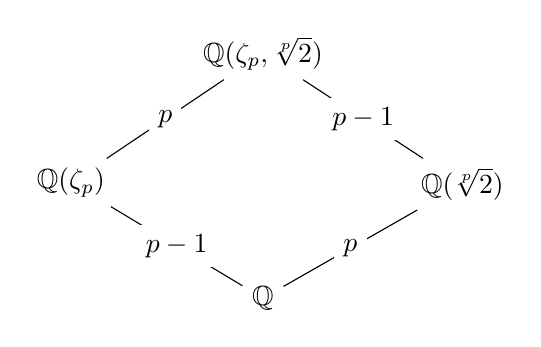
\begin{tikzpicture}[node distance=2cm]
\node(1)			{$\Q(\zeta_p, \sqrt[p]{2})$};
\node(2)			[below left = 1cm and 1cm of 1]
{$\Q(\zeta_p)$};
\node(3)			[below right = 1cm and 1cm of 1]
{$\Q(\sqrt[p]{2})$};
\node(4)			[below = 2.5cm of 1]
{$\Q$};

\draw(1) -- (2) node [midway, fill=white] {$p$};
\draw(1) -- (3) node [midway, fill=white] {$p-1$};
\draw(2) -- (4) node [midway, fill=white] {$p-1$};
\draw(3) -- (4) node [midway, fill=white] {$p$};
\end{tikzpicture}
\end{center}
\end{figure}

\end{proof}

\item (Exercise 9 in DF \S 14.2.) Give (with proof) an example of fields $F_1, F_2, F_3$ with $F_0 := \mathbf{Q} \subset F_1 \subset F_2 \subset F_3$, such that $[F_3:\mathbf{Q}]=8$, $F_2/\mathbf{Q}$ is not Galois, but $F_i/F_j$ is Galois for every $i>j$ other than $(i,j)=(2,0)$.

\begin{proof}

Let $F_1 = \Q(\sqrt{2}), F_2 = \Q(\sqrt[4]{2}), F_3 = \Q(\sqrt[4]{2}, i)$.  Then clearly $\Q \subset F_1 \subset F_2 \subset F_3$.  Also, $F_2 \cong \mathlarger{\mathlarger{\mathlarger{\slfrac{\Q}{(x^4 - 2)}}}}$, which has degree $4$ over $\Q$ because $x^4 - 2$ is irreducible over $\Q$, and $F_3 = F_2(i) \cong \mathlarger{\mathlarger{\mathlarger{\slfrac{F_2}{(x^2 + 1)}}}}$, which has degree $2$ over $F_2$ because $x^2 + 1$ is irreducible over $F_2$.  Thus $[F_3 : \Q] = [F_3 : F_2][F_2 : \Q] = 2 \cdot 4 = 8$.

$F_1$ is the splitting field for the polynomial $x^2 - 2$ over $\Q$.  $F_2$ is the splitting field for the polynomial $x^2 - \sqrt{2}$ over $F_1$.  $F_3$ is the splitting field for the polynomial $x^4 - 2$ over $\Q$, $F_1$, and $F_2$.  Thus, $F_i / F_j$ is Galois for every $i > j$ other than $(i,j) = (2,0)$.

However, $F_2 / \Q$ is not Galois.  Since $F_2$ contains a root of the irreducible polynomial $x^4 - 2$, if it were Galois then it would contain all the roots.  However, it does not contain the root $i\sqrt[4]{2}$.

\end{proof}

\item (Exercise 14 in DF \S 14.2.) Show that $\mathbf{Q}(\sqrt{2+\sqrt{2}})$ is a cyclic quartic field, i.e., is a Galois extension of degree $4$ over $\mathbf{Q}$ with cyclic Galois group.

\begin{proof}

First, note that $\sqrt{2 + \sqrt{2}}$ is a root of $p(x) = x^4 - 4x^2 + 2$:
\begin{align*}
p \left( \sqrt{2 + \sqrt{2}} \right) &= \left( \sqrt{2 + \sqrt{2}} \right) ^4 - 4 \left( \sqrt{2 + \sqrt{2}} \right) ^2 + 2
\\
&= \left(2 + \sqrt{2} \right)^2 - 4 \left(2 + \sqrt{2} \right) + 2
\\
&= 6 + 4\sqrt{2} - 8 - 4\sqrt{2} + 2
\\
&= 0.
\end{align*}
Also, $p(x)$ is irreducible over $\Q$ by Eisenstein's criterion, since $2 \mid 2$ and $2 \mid 4$, but $2^2 \nmid 1$.  We can also check that $\sqrt{2 - \sqrt{2}}$ is a root:
\begin{align*}
p \left( \sqrt{2 - \sqrt{2}} \right) &= \left( \sqrt{2 - \sqrt{2}} \right) ^4 - 4 \left( \sqrt{2 - \sqrt{2}} \right) ^2 + 2
\\
&= \left(2 - \sqrt{2} \right)^2 - 4 \left(2 - \sqrt{2} \right) + 2
\\
&= 6 - 4\sqrt{2} - 8 + 4\sqrt{2} + 2
\\
&= 0.
\end{align*}
Since $p(x)$ is an even function, the other two roots are $-\sqrt{2 + \sqrt{2}}$ and $-\sqrt{2 - \sqrt{2}}$.  Therefore, if we can show that $\sqrt{2 - \sqrt{2}} \in \Q(\sqrt{2 + \sqrt{2}})$, we will have shown that the extension is a splitting field for the separable polynomial $p(x)$, thus it is Galois, since it will necessarily contain the negative roots as well by closure.

Note that
$$
\dfrac{\sqrt{2 - \sqrt{2}}}{\sqrt{2 + \sqrt{2}}} = \dfrac{\sqrt{2 - \sqrt{2}}}{\sqrt{2 + \sqrt{2}}} \cdot \dfrac{\sqrt{2 + \sqrt{2}}}{\sqrt{2 + \sqrt{2}}} = \dfrac{\sqrt{4-2}}{2 + \sqrt{2}} = \dfrac{\sqrt{2}}{2 + \sqrt{2}} \cdot \dfrac{2 - \sqrt{2}}{2 - \sqrt{2}}
$$
$$
= \dfrac{2\sqrt{2} - 2}{4-2} = \dfrac{2\sqrt{2} - 2}{2} = \sqrt{2} - 1.
$$
Also, $\left( \sqrt{2 + \sqrt{2}} \right)^2 - 3 = 2 + \sqrt{2} - 3 = \sqrt{2} - 1 \in \Q(\sqrt{2 + \sqrt{2}})$.  Therefore, $\sqrt{2 - \sqrt{2}} = (\sqrt{2} - 1)\sqrt{2 + \sqrt{2}} = \in \Q(\sqrt{2 + \sqrt{2}})$.  So $\Q(\sqrt{2 + \sqrt{2}})$ is Galois.

Since the Galois group has order 4, and there are 4 possible images for any given root, it must be that the action of an automorphism $\sigma$ on one root determines the entire map.  So consider the action of $\sigma$ on the root $\sqrt{2 + \sqrt{2}}$.

First, note that $$\left(\sqrt{2 + \sqrt{2}}\right)\left(\sqrt{2 - \sqrt{2}}\right) = \sqrt{2}.$$

Now, define $\sigma$ by $\sqrt{2 + \sqrt{2}} \mapsto \sqrt{2 - \sqrt{2}}$.  Then $\left(\sqrt{2 + \sqrt{2}}\right)^2 = 2 + \sqrt{2} \mapsto 2 + \sigma(\sqrt{2}) = \left(\sqrt{2 - \sqrt{2}}\right)^2 = 2 - \sqrt{2}$, so $\sqrt{2} \mapsto -\sqrt{2}$.  Thus,
$$
\sigma\left(\sqrt{2 - \sqrt{2}}\right) =  \dfrac{\sigma\left(\sqrt{2 + \sqrt{2}}\right)}{\sigma(\sqrt{2})} = \dfrac{\sqrt{2 - \sqrt{2}}}{-\sqrt{2}} = - \sqrt{2 + \sqrt{2}}.
$$

So $\sigma$ rotates the roots of $p(x)$.  Therefore, it cannot be that $\sigma^2$ is the identity, since $\sigma^2(\sqrt{2 + \sqrt{2}}) = \sigma(\sqrt{2 - \sqrt{2}} = -\sqrt{2 + \sqrt{2}}$.  Since $\sigma$ is nontrivial and does not have order 2, it must have order 4.  So $\Gal\left(\Q\left(\sqrt{2 + \sqrt{2}}\right)\right)$ contains an element of order 4, thus it is a cyclic group of order 4.
\end{proof}

\item (Adapted from Exercise 17 in DF \S 14.2.) Let $K/F$ be a (finite) Galois extension.  For each $\alpha \in K$, define the \emph{norm} of $\alpha$ to be 
\[
N_{K/F}(\alpha) = \prod_{\sigma \in \Gal (K/F)} \sigma(\alpha) \text{.}
\]

(a) Prove that $N_{K/F}(\alpha) \in F$ for any $\alpha \in K$.

\begin{proof}

Let $\tau \in \Gal(K/F)$.  Then $\tau$ acts on $\Gal(K/F)$ as a permutation.  Therefore, as a group action, $\tau : \Gal(K/F) \rightarrow \Gal(K/F)$ is a bijection.  Thus $\{\tau \circ \sigma : \sigma \in \Gal(K/F)\} = \Gal(K/F)$.  So
$$
\tau \left( N_{K/F}(\alpha) \right) = \tau \left(\prod_{\sigma \in \Gal (K/F)} \sigma(\alpha) \right) = \prod_{\sigma \in \Gal (K/F)} \tau \circ \sigma(\alpha)
= \prod_{\sigma \in \Gal (K/F)} \sigma(\alpha) = N_{K/F}(\alpha).
$$

Since an arbitrary $\tau \in \Gal(K/F)$ fixes the $N_{K/F}(\alpha)$, we know that $N_{K/F}(\alpha)$ is in the fixed field of $\Gal(K/F)$, which is $F$.

\end{proof}

(b) Prove that $N_{K/F}(\alpha \beta) = N_{K/F}(\alpha) N_{K/F}(\beta)$ for any $\alpha,\beta \in K$.

\begin{proof}

This follows easily from the fact that $\sigma$ is an automorphism.
\begin{align*}
N_{K/F}(\alpha\beta) &= \prod_{\sigma \in \Gal (K/F)} \sigma(\alpha\beta) = \prod_{\sigma \in \Gal (K/F)} \sigma(\alpha)\sigma(\beta)
\\
&= \prod_{\sigma \in \Gal (K/F)} \sigma(\alpha) \prod_{\sigma \in \Gal (K/F)} \sigma(\beta)
= N_{K/F}(\alpha)N_{K/F}(\beta)
\end{align*}
\end{proof}

(c) Assume in addition that $[K:F]=2$.  Show that there exists $\gamma \in K$ such that $K = F(\gamma)$ and $\gamma^2 \in F$.  Let $D=\gamma^2$.  Show that for any $a,b \in F$, $N_{K/F}(a+b\gamma) = a^2-Db^2$.

\begin{proof}

For the first part, we need to assume that $F$ has characteristic $>2$.  Let $p(x) = ax^2 + bx + c$ be the minimum polynomial of $\alpha$.  Then some $\alpha \in K$ is a root of $p(x)$.  So $\alpha^2 = \dfrac{b\alpha + c}{a}$.

Let $\gamma = 2a\alpha + b$.  Since $\gamma \in K$, we know that $F(\gamma) \subseteq K$.  Since the field has characteristic greater than 2, we have $\alpha = \dfrac{\gamma - b}{2a} \in F(\gamma)$, so $K \subseteq F(\gamma)$.  Thus $K = F(\alpha)$.  Also, $\gamma^2 = 4a^2 \alpha^2 + 4ab\alpha + b^2 = 4a^2\left( \dfrac{b\alpha + c}{a}\right) + 4ab\alpha + b^2 = b^2 - 4ac \in F$.  So $D = b^2 - 4ac$ suffices.

Now, let $a$ and $b$ be arbitrary elements of $F$.  Note that $a + b\gamma$ and $a - b\gamma$ are roots of the separable polynomial $x^2 - 2ax + a^2 - Db^2$.  Since these roots are not in $F$, the polynomial is irreducible.  Thus the Galois group of $K$ must permute its roots.

Since $\Gal(K/F)$ has order 2, and the automorphisms are defined by their action on $\gamma$, the only nontrivial automorphism is the one that takes $a + b\gamma$ to $a - b\gamma$.  Therefore,

$$
N_{K/F}(a + b\gamma) = \prod_{\sigma \in \Gal (K/F)} \sigma(a + b\gamma) = (a+b\gamma)(a-b\gamma) = a^2 - \gamma^2b^2 = a^2 - Db^2.
$$

\end{proof}

(d) Given $\alpha \in K$, let $m_\alpha (X) = X^d + a_{d-1}X^{d-1} + \ldots + a_1 X + a_0 \in F[X]$ be the minimal polynomial for $\alpha$ over $F$.  Let $n=[K:F]$.  Prove that (i) $d$ divides $n$, (ii) there are $d$ distinct Galois conjugates of $\alpha$ (that is, the set $\{\sigma(\alpha): \sigma \in \Gal(K/F)\}$ has $d$ elements), and (iii) each Galois conjugate (i.e. each element of the aforementioned set) appears $n/d$ times in the product defining $N_{K/F}(\alpha)$.  Deduce that $N_{K/F}(\alpha) = (-1)^n a_0^{n/d}$.

(Hint: for (iii), use the Galois correspondence (Theorem 14 in \S 14.2).)

\begin{proof}

It is clear that $d$ divides $n$.  $d$ is, by definition, the degree of the extension $F(\alpha)$, and $F \subseteq F(\alpha) \subseteq K$.  So by corollary 15 on pg. 524, $d$ must divide $n$.

Let $\sigma \in \Gal(K/F) = G$.  By Theorem 13, $m_{\alpha}$ is separable, and thus has distinct roots $\alpha_1, \dots , \alpha_d \in K$, where $\alpha_1 = \alpha$.  We can now construct an automorphism $\sigma$ that takes $\alpha$ to any arbitrary $\alpha_i$:

Define a homomorphism $\sigma$ fixing $F$ on $F(\alpha,\alpha_i)$ partially by $\sigma(\alpha) = \alpha_i$, so that $\sigma(a_0 + a_1 \alpha + \cdots + a_d \alpha^d) = a_0 + a_1 \alpha_i + \cdots + a_d \alpha_i^d$.  If $\alpha_i$ is generated by $\alpha$ over $F$, then $\sigma$ is completely defined on $F(\alpha,\alpha_i)$.  Otherwise, if $\alpha_i$ is not generated by $\alpha$ over $F$, then define $\sigma(\alpha_i) = \alpha$.  This cannot contradict the fact that $\sigma$ is a homomorphism, since its action on $\alpha_i$ was undetermined.  By Theorem 13.27, we know that $\sigma$ can be extended to an automorphism $\tau$ on all of $K$, since $K$ is the splitting field of some polynomial over $F(\alpha,\alpha_i)$.  Therefore, $\tau \in \Gal(K/F)$ takes $\alpha$ to an arbitrary $\alpha_i$, thus every $\alpha_i$ is a conjugate of $\alpha$.

Let $E = F(\alpha_1, \dots , \alpha_d)$, and let $H = \Gal(E/F)$ (since $E$ is the splitting field for the separable polynomial $m_{\alpha}(x)$, we know it is Galois).  By part (iii) of Galois correspondence, $\Gal(E/F) \cong G/H$, thus $|\Gal(E/F)| = \dfrac{|G|}{|H|} = \dfrac{n}{d}$.  By the statements in the proof of Galois correspondence, two automorphisms $\sigma_1, \sigma_2 \in G$ restrict to the same embedding of $E$ if and only if they are representatives of the same coset of $H$ in $G$.  Each coset contains $n/d$ elements, and there are $d$ cosets.  Let $H_1, \dots , H_d$ be these cosets, where $H_i$ is such that $\sigma(\alpha) = \alpha_i$ for all $\sigma \in H_i$.  Then we have

$$
N_{K/F}(\alpha) = \prod_{\sigma \in \Gal (K/F)} \sigma(\alpha) = \prod_{i=1}^d \prod_{\sigma \in H_i} \sigma(\alpha) = \prod_{i=1}^d \alpha_i^{n/d}
$$
since there are $n/d$ elements in $H_i$, all of which map $\alpha$ to $\alpha_i$.  So each $\alpha_i$ appears $n/d$ times in the product.

Now, the minimal polynomial of $\alpha$ can be expanded as 
\begin{align*}
m_{\alpha}(x) &= (x - \alpha_1)\cdots(x-\alpha_d)
\\
&= x^d + a_{d-1}x^{d-1} + \cdots + a_1x + (-1)^d\prod_{i=1}^d \alpha_i
\\
&= x^d + a_{d-1}x^{d-1} + \cdots + a_1x + a_0
\end{align*}
therefore $a_0 = (-1)^d\prod_{i=1}^d \alpha_i$, thus dividing by $(-1)^d$ gives $\prod_{i=1}^d \alpha_i = (-1)^d a_0$.  So $$N_{K/F}(\alpha) = \prod_{i=1}^d \alpha_i^{n/d} = \left( \prod_{i=1}^d \alpha_i \right)^{n/d} = ((-1)^d a_0)^{n/d} = (-1)^n (a_0)^{n/d}.$$

\end{proof}

\end{enumerate}
\end{document}
